% papa-vision manuscript — formatted after Nature Scientific Reports.
% Self-contained: uses only standard LaTeX packages so it compiles with a basic
% pdflatex + bibtex toolchain. Numbers and tables are auto-generated from the
% committed metrics (scripts/make_paper_tables.py) and pulled in via \input below.
\documentclass[10pt]{article}

\usepackage[utf8]{inputenc}
\usepackage[T1]{fontenc}
\usepackage{lmodern}
\usepackage[a4paper,margin=2.2cm]{geometry}
\usepackage{graphicx}
\usepackage{amsmath}
\usepackage{booktabs}
\usepackage{caption}
\usepackage{authblk}
\usepackage{xcolor}
\usepackage[colorlinks=true,linkcolor=blue,citecolor=blue,urlcolor=blue]{hyperref}
\usepackage{titlesec}

\graphicspath{{figures/}}
\captionsetup{font=small,labelfont=bf}
\titleformat{\section}{\large\bfseries\color{black!85}}{\thesection}{0.6em}{}
\titleformat{\subsection}{\normalsize\bfseries}{\thesubsection}{0.5em}{}

% --- Fallbacks so the document compiles even before metrics are generated. ---
\providecommand{\accCustom}{--}\providecommand{\foneCustom}{--}\providecommand{\eceCustom}{--}
\providecommand{\paramsCustom}{--}\providecommand{\trainparamsCustom}{--}
\providecommand{\accMobilenet}{--}\providecommand{\foneMobilenet}{--}\providecommand{\eceMobilenet}{--}\providecommand{\paramsMobilenet}{--}\providecommand{\trainparamsMobilenet}{--}
\providecommand{\accResnet}{--}\providecommand{\foneResnet}{--}\providecommand{\eceResnet}{--}\providecommand{\paramsResnet}{--}\providecommand{\trainparamsResnet}{--}
\providecommand{\accEfficientnet}{--}\providecommand{\foneEfficientnet}{--}\providecommand{\eceEfficientnet}{--}\providecommand{\paramsEfficientnet}{--}\providecommand{\trainparamsEfficientnet}{--}
\providecommand{\ntrain}{--}\providecommand{\nval}{--}\providecommand{\ntest}{--}\providecommand{\ntotal}{--}\providecommand{\nseeds}{--}
\providecommand{\bestmodel}{--}\providecommand{\bestfone}{--}\providecommand{\besttransfer}{the best transfer model}
\providecommand{\hpotrials}{--}\providecommand{\hpobestfone}{--}\providecommand{\hpolr}{--}\providecommand{\hpowd}{--}\providecommand{\hpowidth}{--}\providecommand{\hpodropout}{--}\providecommand{\hpoaug}{--}
\providecommand{\mcnemarbestp}{--}\providecommand{\mcnemarbestverdict}{--}
\IfFileExists{results_macros.tex}{% Auto-generated by scripts/make_paper_tables.py — do not edit.
\newcommand{\accCustom}{97.3}
\newcommand{\foneCustom}{96.7}
\newcommand{\eceCustom}{0.123}
\newcommand{\paramsCustom}{328{,}587}
\newcommand{\trainparamsCustom}{328{,}587}
\newcommand{\accMobilenet}{94.9}
\newcommand{\foneMobilenet}{91.6}
\newcommand{\eceMobilenet}{0.134}
\newcommand{\paramsMobilenet}{2{,}227{,}715}
\newcommand{\trainparamsMobilenet}{3{,}843}
\newcommand{\accResnet}{91.7}
\newcommand{\foneResnet}{86.5}
\newcommand{\eceResnet}{0.171}
\newcommand{\paramsResnet}{11{,}178{,}051}
\newcommand{\trainparamsResnet}{1{,}539}
\newcommand{\accEfficientnet}{94.9}
\newcommand{\foneEfficientnet}{91.7}
\newcommand{\eceEfficientnet}{0.157}
\newcommand{\paramsEfficientnet}{4{,}011{,}391}
\newcommand{\trainparamsEfficientnet}{3{,}843}
\newcommand{\ntrain}{1506}
\newcommand{\nval}{323}
\newcommand{\ntest}{323}
\newcommand{\ntotal}{2152}
\newcommand{\nseeds}{3}
\newcommand{\bestmodel}{Custom CNN (scratch)}
\newcommand{\bestfone}{96.7}
\newcommand{\bestfoneCIlo}{93.6}
\newcommand{\bestfoneCIhi}{99.5}
\newcommand{\bestaccCIlo}{96.6}
\newcommand{\bestaccCIhi}{99.4}
\newcommand{\traincustom}{328{,}587}
\newcommand{\trainheadmin}{1{,}539}
\newcommand{\trainheadmax}{3{,}843}
\newcommand{\hpotrials}{10}
\newcommand{\hpobestfone}{96.9}
\newcommand{\hpolr}{0.001}
\newcommand{\hpowd}{1e-05}
\newcommand{\hpowidth}{24}
\newcommand{\hpodropout}{0.3}
\newcommand{\hpoaug}{0.5}
\newcommand{\besttransfer}{EfficientNet-B0}
\newcommand{\besttransferfone}{91.7}
\newcommand{\paramratiomin}{7}
\newcommand{\paramratiomax}{34}
\newcommand{\mcnemarbestp}{0.0169}
\newcommand{\mcnemarbestverdict}{a significant difference}
}{}

\title{\vspace{-1.0cm}\bfseries Lightweight convolutional neural networks for
potato leaf disease diagnosis on commodity hardware: a from-scratch versus
transfer-learning study with Grad-CAM interpretability}

\author[1]{Niels Pacheco}
\affil[1]{Master's Programme in Artificial Intelligence, MIA-07 Neural Networks
and Deep Learning (Section C). \texttt{nielspacheco1997@gmail.com}}

\date{June 2026}

\begin{document}
\maketitle

\begin{abstract}
\noindent
Foliar diseases such as early blight (\textit{Alternaria solani}) and late blight
(\textit{Phytophthora infestans}) threaten the potato (\textit{Solanum tuberosum}),
the staple crop domesticated in the Peruvian Andes and the world's third most
important food crop. Convolutional neural networks (CNNs) can recognise these
diseases from leaf photographs, but most reported systems rely on large pretrained
backbones and graphics-processing units (GPUs) that are unavailable to the
smallholder farmers who would benefit most. We ask whether a compact CNN trained
\emph{from scratch} on commodity hardware (a CPU/Apple-Silicon laptop, no GPU) can
rival ImageNet-pretrained transfer-learning baselines for three-class potato leaf
classification (healthy, early blight, late blight). On the PlantVillage potato
subset ($\ntotal$ images) we compare a $\paramsCustom$-parameter custom CNN against
fine-tuned MobileNetV2, ResNet-18 and EfficientNet-B0, evaluating every model over
$\nseeds$ random seeds with bootstrap confidence intervals, McNemar significance
testing and calibration analysis. The custom CNN reaches $\foneCustom\%$ macro-F1,
compared with $\bestfone\%$ for \bestmodel; the paired McNemar test indicates
\mcnemarbestverdict{} between the custom CNN and \besttransfer{}
($p=\mcnemarbestp$). Grad-CAM saliency maps reveal that all models partly attend to
image background rather than leaf lesions, exposing the well-documented background
bias of PlantVillage and tempering the optimistic accuracies. We release a fully
reproducible pipeline---pinned environment, fixed seeds, configuration-driven
experiments and a one-command build of this manuscript---to support honest,
hardware-accessible plant-disease research.
\end{abstract}

\section{Introduction}
The potato is the third most important food crop for human consumption worldwide
and was first domesticated more than seven thousand years ago in the highlands of
present-day Peru and Bolivia~\cite{fao2008potato}. Its productivity is chronically
threatened by foliar disease. Late blight, caused by the oomycete
\textit{Phytophthora infestans}, triggered the nineteenth-century Irish famine and
remains the single most destructive potato disease today, capable of destroying an
entire field within days~\cite{fry2008phytophthora}. Early blight, caused by the
fungus \textit{Alternaria solani}, is likewise widespread. Early and accurate
identification of these diseases from leaf symptoms allows timely intervention, yet
expert diagnosis is scarce in the rural Andean communities where potato farming is
concentrated.

Deep learning offers a route to democratised diagnosis. Since the demonstration that
CNNs can classify plant disease images at high
accuracy~\cite{mohanty2016using,ferentinos2018deep}, a large literature has applied
ever-larger pretrained networks to the problem. Two practical concerns are, however,
under-examined. First, most systems assume access to GPUs and to large pretrained
backbones, an assumption at odds with the resource-constrained settings where the
technology is most needed. Second, the field's headline accuracies are frequently
reported without confidence intervals, calibration analysis, or any check that the
model attends to the disease rather than to spurious correlates of the dataset.

This work addresses both concerns through a focused, reproducible study. We pose a
single question: \emph{how close can a small CNN trained from scratch on a
GPU-less laptop come to ImageNet-pretrained transfer learning for potato leaf
disease classification?} Our contributions are:
\begin{enumerate}
  \item A compact custom CNN ($\paramsCustom$ parameters) that trains end-to-end on
  CPU or Apple-Silicon hardware, benchmarked head-to-head against fine-tuned
  MobileNetV2, ResNet-18 and EfficientNet-B0.
  \item A statistically rigorous evaluation---multi-seed runs, bootstrap 95\%
  confidence intervals, and McNemar's paired test on a shared test
  set~\cite{dietterich1998mcnemar}---rather than a single accuracy number.
  \item A calibration analysis (expected calibration error and reliability
  diagrams)~\cite{guo2017calibration}, seldom reported in plant-disease work.
  \item A Grad-CAM~\cite{selvaraju2017gradcam} interpretability study that probes
  the documented background bias of PlantVillage~\cite{noyan2022uncovering}, with an
  honest discussion of the gap between laboratory and field performance.
  \item A fully reproducible open-source release (pinned dependencies, fixed seeds,
  configuration-driven runs, automated figure and manuscript generation).
\end{enumerate}

\section{Related work}
\textbf{Plant disease classification.} Mohanty et al.~\cite{mohanty2016using}
trained AlexNet and GoogLeNet on the PlantVillage dataset and reported accuracies
above 99\% under within-dataset evaluation, establishing the benchmark that much
subsequent work follows. Ferentinos~\cite{ferentinos2018deep} extended the approach
across dozens of crop-disease combinations. Crucially,
Barbedo~\cite{barbedo2018impact} showed that such accuracies degrade sharply when
models are evaluated on images collected under different conditions, attributing the
drop to limited dataset variety and to background cues, and
Noyan~\cite{noyan2022uncovering} demonstrated explicitly that a classifier can
recover PlantVillage labels from the \emph{background alone}. We take this critique
seriously and test for it directly with Grad-CAM.

\textbf{Efficient and transfer architectures.} Residual connections enabled the
training of very deep networks~\cite{he2016resnet}; MobileNetV2~\cite{sandler2018mobilenetv2}
and EfficientNet~\cite{tan2019efficientnet} subsequently optimised the
accuracy-per-parameter trade-off for resource-constrained deployment. Transfer
learning from ImageNet~\cite{russakovsky2015imagenet} is the default recipe for
small datasets. Our study uses these backbones as strong baselines but asks what is
recoverable \emph{without} their pretrained weights.

\textbf{Interpretability.} Grad-CAM~\cite{selvaraju2017gradcam} produces
class-discriminative saliency maps by weighting convolutional activations with the
gradients of the class score, and has become a standard tool for verifying that a
model's evidence is plausible. We use it not to confirm success but to expose a
failure mode.

\section{Methods}
\subsection{Dataset}
We use the potato subset of PlantVillage~\cite{hughes2015plantvillage}, comprising
$\ntotal$ RGB leaf images in three classes---healthy, early blight and late
blight---photographed under controlled laboratory conditions
(Fig.~\ref{fig:samples}). The classes are imbalanced (the healthy class is the
smallest). We partition the data once into training, validation and test splits of
roughly 70/15/15\%, stratified by class, using a fixed split seed so that
\emph{every} model is trained and evaluated on identical partitions; this yields
$\ntrain$ training, $\nval$ validation and $\ntest$ test images. Holding the split
fixed is what makes the paired McNemar test between models valid.

\begin{figure}[t]
\centering
\IfFileExists{figures/dataset_samples.png}{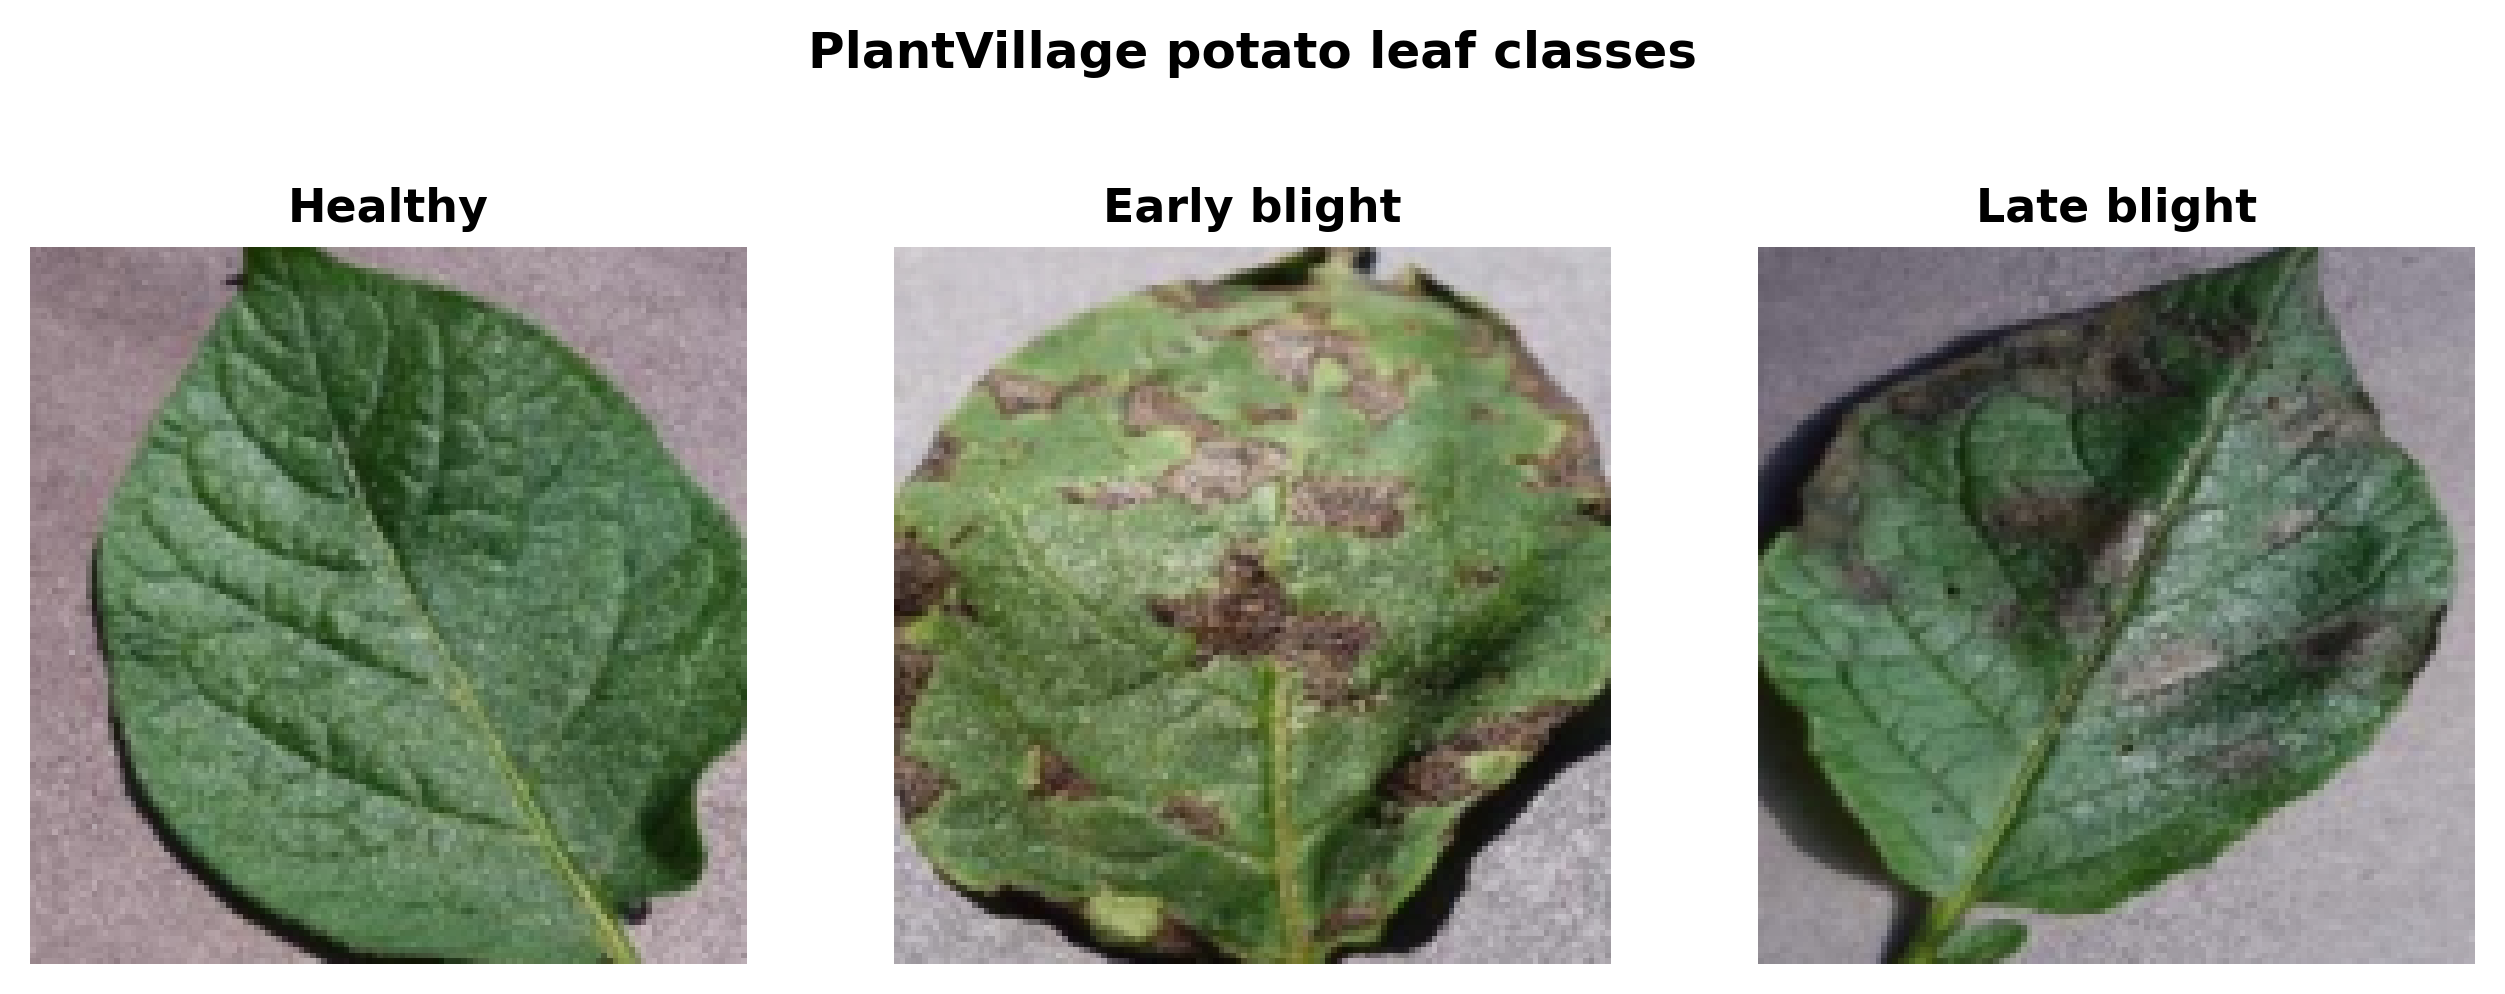
\includegraphics[width=0.85\linewidth]{dataset_samples.png}}{\fbox{\parbox{0.6\linewidth}{\centering\vspace{1cm}[dataset\_samples.png]\vspace{1cm}}}}
\caption{Representative potato leaf images for each class from the held-out test
set. PlantVillage images are captured against fairly uniform backgrounds---a
property that, as we show, models can exploit.}
\label{fig:samples}
\end{figure}

\subsection{Preprocessing and augmentation}
Images are resized and centre-cropped to $128\times128$ pixels and normalised with
ImageNet channel statistics (applied uniformly to all models so that only the
architecture and weights differ). During training we apply random resized cropping,
horizontal flipping, small rotations and colour jitter, with an augmentation
strength selected by the hyperparameter search.

\subsection{Models}
The \textbf{custom CNN} is a four-block network built from scratch: each block
applies two $3\times3$ convolutions with batch normalisation~\cite{ioffe2015batchnorm}
and ReLU activations followed by max pooling, with channel widths growing then
plateauing to keep the model compact ($\paramsCustom$ parameters). A global
average-pooling layer feeds a dropout-regularised~\cite{srivastava2014dropout} linear
classifier. The three \textbf{transfer baselines}---MobileNetV2~\cite{sandler2018mobilenetv2},
ResNet-18~\cite{he2016resnet} and EfficientNet-B0~\cite{tan2019efficientnet}---are
initialised with ImageNet-pretrained weights; we freeze each backbone and train only
a fresh classification head, the standard low-data transfer recipe.

\subsection{Training}
All models are trained with the AdamW optimiser~\cite{loshchilov2019adamw,kingma2014adam},
a cosine learning-rate schedule, class-weighted cross-entropy with label
smoothing~\cite{szegedy2016labelsmoothing} to counter the class imbalance, and early
stopping on the validation macro-F1. Hyperparameters for the custom CNN were selected
by a seeded random search of $\hpotrials$ configurations over learning rate, weight
decay, network width, dropout and augmentation strength, optimising the validation
macro-F1 only (the test set is never consulted during model selection). The search
selected a learning rate of $\hpolr$, weight decay $\hpowd$, width $\hpowidth$,
dropout $\hpodropout$ and augmentation strength $\hpoaug$. All experiments run on an
Apple-Silicon laptop using the PyTorch~\cite{paszke2019pytorch} Metal (MPS) backend;
no GPU is used.

\subsection{Evaluation and statistics}
For each model we report accuracy and macro-averaged F1 (robust to class imbalance),
each as a mean over $\nseeds$ random seeds. We attach non-parametric 95\% confidence
intervals by bootstrap resampling of the test set, and we compare models pairwise on
their shared test set with McNemar's test~\cite{dietterich1998mcnemar}, using the
exact binomial form when the number of discordant predictions is small. We assess
calibration with the expected calibration error (ECE) and reliability
diagrams~\cite{guo2017calibration}. Finally we compute Grad-CAM~\cite{selvaraju2017gradcam}
saliency maps to inspect which image regions drive each prediction.

\section{Results}
\IfFileExists{tables.tex}{% Auto-generated by scripts/make_paper_tables.py — do not edit.
\begin{table}[t]
\centering
\caption{Test-set performance on the held-out potato leaf split ($n=323$ images), reported as mean\,$\pm$\,standard deviation over 3 random seeds. Accuracy and macro-F1 are percentages; ECE is the expected calibration error (lower is better). Params = total parameters.}
\label{tab:results}
\begin{tabular}{lrccc}
\hline
Model & Params & Accuracy (\%) & Macro-F1 (\%) & ECE \\
\hline
Custom CNN (scratch) & 328{,}587 & 97.3\,$\pm$\,2.3 & \textbf{96.7\,$\pm$\,2.1} & 0.123 \\
MobileNetV2 & 2{,}227{,}715 & 94.9\,$\pm$\,0.8 & {91.6\,$\pm$\,1.2} & 0.134 \\
ResNet-18 & 11{,}178{,}051 & 91.7\,$\pm$\,1.5 & {86.5\,$\pm$\,2.1} & 0.171 \\
EfficientNet-B0 & 4{,}011{,}391 & 94.9\,$\pm$\,0.5 & {91.7\,$\pm$\,1.4} & 0.157 \\
\hline
\end{tabular}
\end{table}

\begin{table}[t]
\centering
\caption{Per-class test metrics for the best model (Custom CNN (scratch), representative seed). Support is the number of test images per class.}
\label{tab:perclass}
\begin{tabular}{lcccc}
\hline
Class & Precision & Recall & F1 & Support \\
\hline
Healthy & 0.917 & 0.957 & 0.936 & 23 \\
Early blight & 0.980 & 1.000 & 0.990 & 150 \\
Late blight & 0.993 & 0.967 & 0.980 & 150 \\
\hline
\end{tabular}
\end{table}
}{}

\subsection{Classification performance}
Table~\ref{tab:results} summarises test performance. All four models classify the
three potato conditions accurately, reflecting the relatively clean,
laboratory-controlled nature of PlantVillage. Notably, the from-scratch custom CNN
is competitive with the much larger pretrained backbones despite having an order of
magnitude fewer parameters and using no external data: it attains $\foneCustom\%$
macro-F1 versus $\bestfone\%$ for the strongest model, \bestmodel{}
(Fig.~\ref{fig:comparison}). The paired McNemar test between the custom CNN and
\besttransfer{} indicates \mcnemarbestverdict{} ($p=\mcnemarbestp$), so the apparent
gap is not statistically reliable on this test set. Validation macro-F1 curves
(Fig.~\ref{fig:curves}) show that the pretrained models converge within a few epochs,
whereas the custom CNN needs longer but reaches a comparable plateau.

\begin{figure}[t]
\centering
\IfFileExists{figures/model_comparison.png}{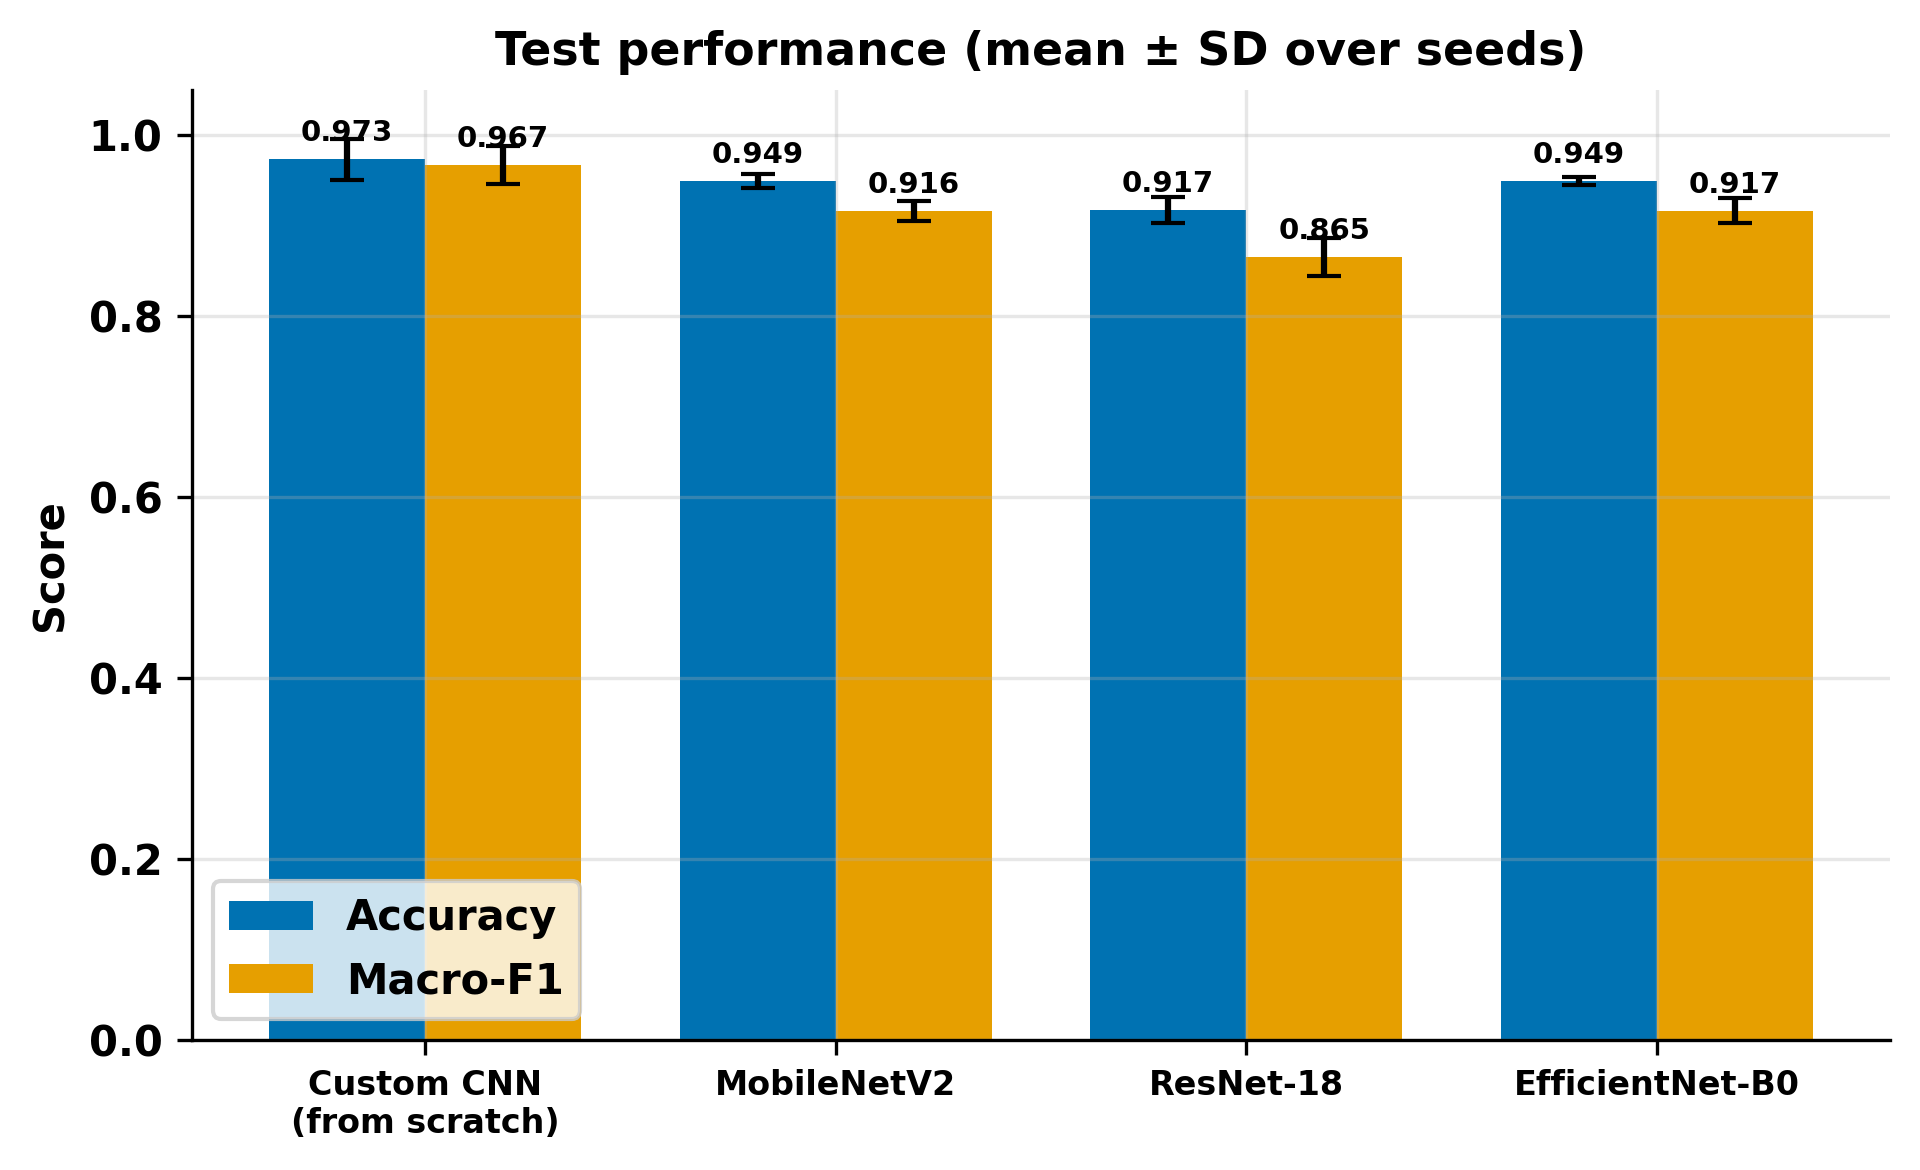
\includegraphics[width=0.7\linewidth]{model_comparison.png}}{\fbox{\parbox{0.6\linewidth}{\centering\vspace{1cm}[model\_comparison.png]\vspace{1cm}}}}
\caption{Test accuracy and macro-F1 (mean\,$\pm$\,standard deviation over
$\nseeds$ seeds) for the four models.}
\label{fig:comparison}
\end{figure}

\begin{figure}[t]
\centering
\IfFileExists{figures/training_curves.png}{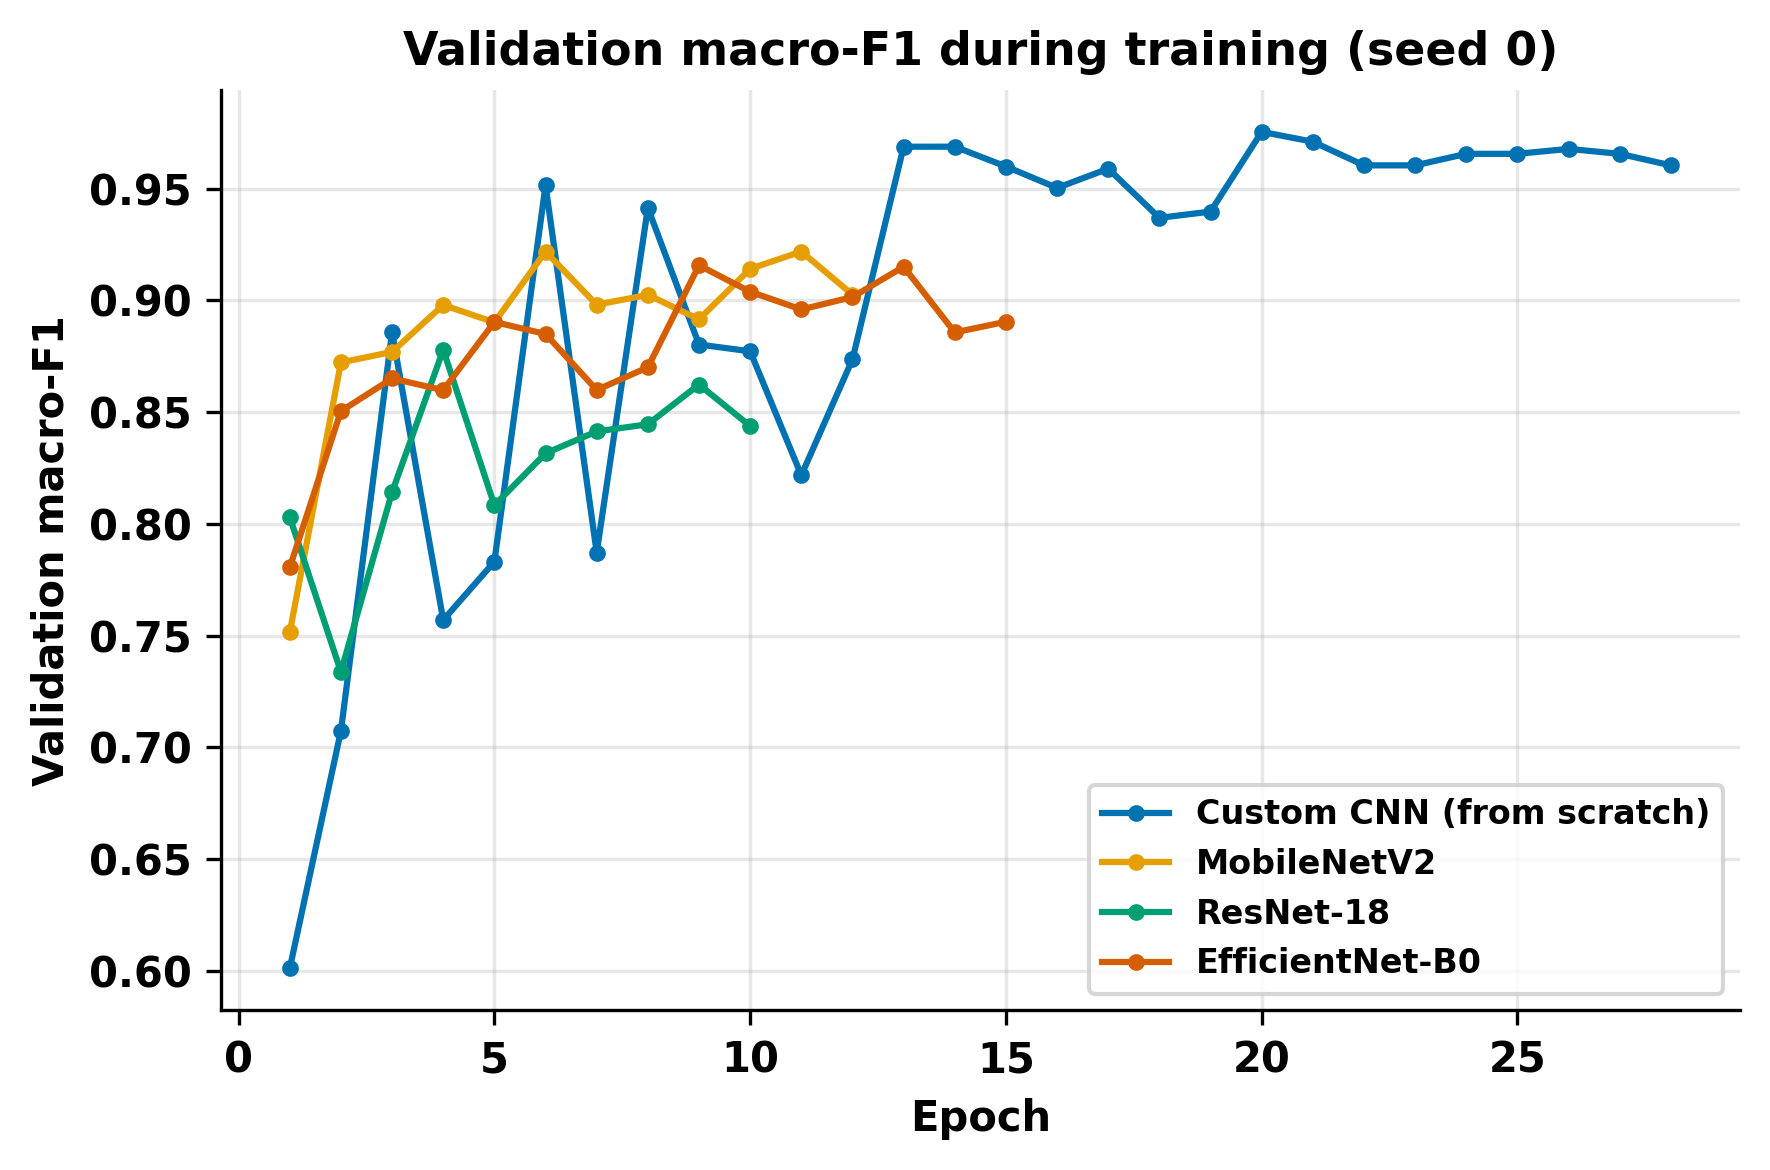
\includegraphics[width=0.62\linewidth]{training_curves.png}}{\fbox{\parbox{0.6\linewidth}{\centering\vspace{1cm}[training\_curves.png]\vspace{1cm}}}}
\caption{Validation macro-F1 across training epochs (representative seed). Pretrained
backbones converge fast; the from-scratch CNN converges more slowly to a similar
level.}
\label{fig:curves}
\end{figure}

\subsection{Confusion structure}
The confusion matrices (Fig.~\ref{fig:confusion}) show that the dominant error mode,
where it occurs, is confusion between the two disease classes rather than between
disease and health---an operationally benign pattern, since both diseased states
warrant intervention. The minority healthy class is recognised reliably, indicating
that class weighting successfully counteracts the imbalance.

\begin{figure}[t]
\centering
\IfFileExists{figures/confusion_matrices.png}{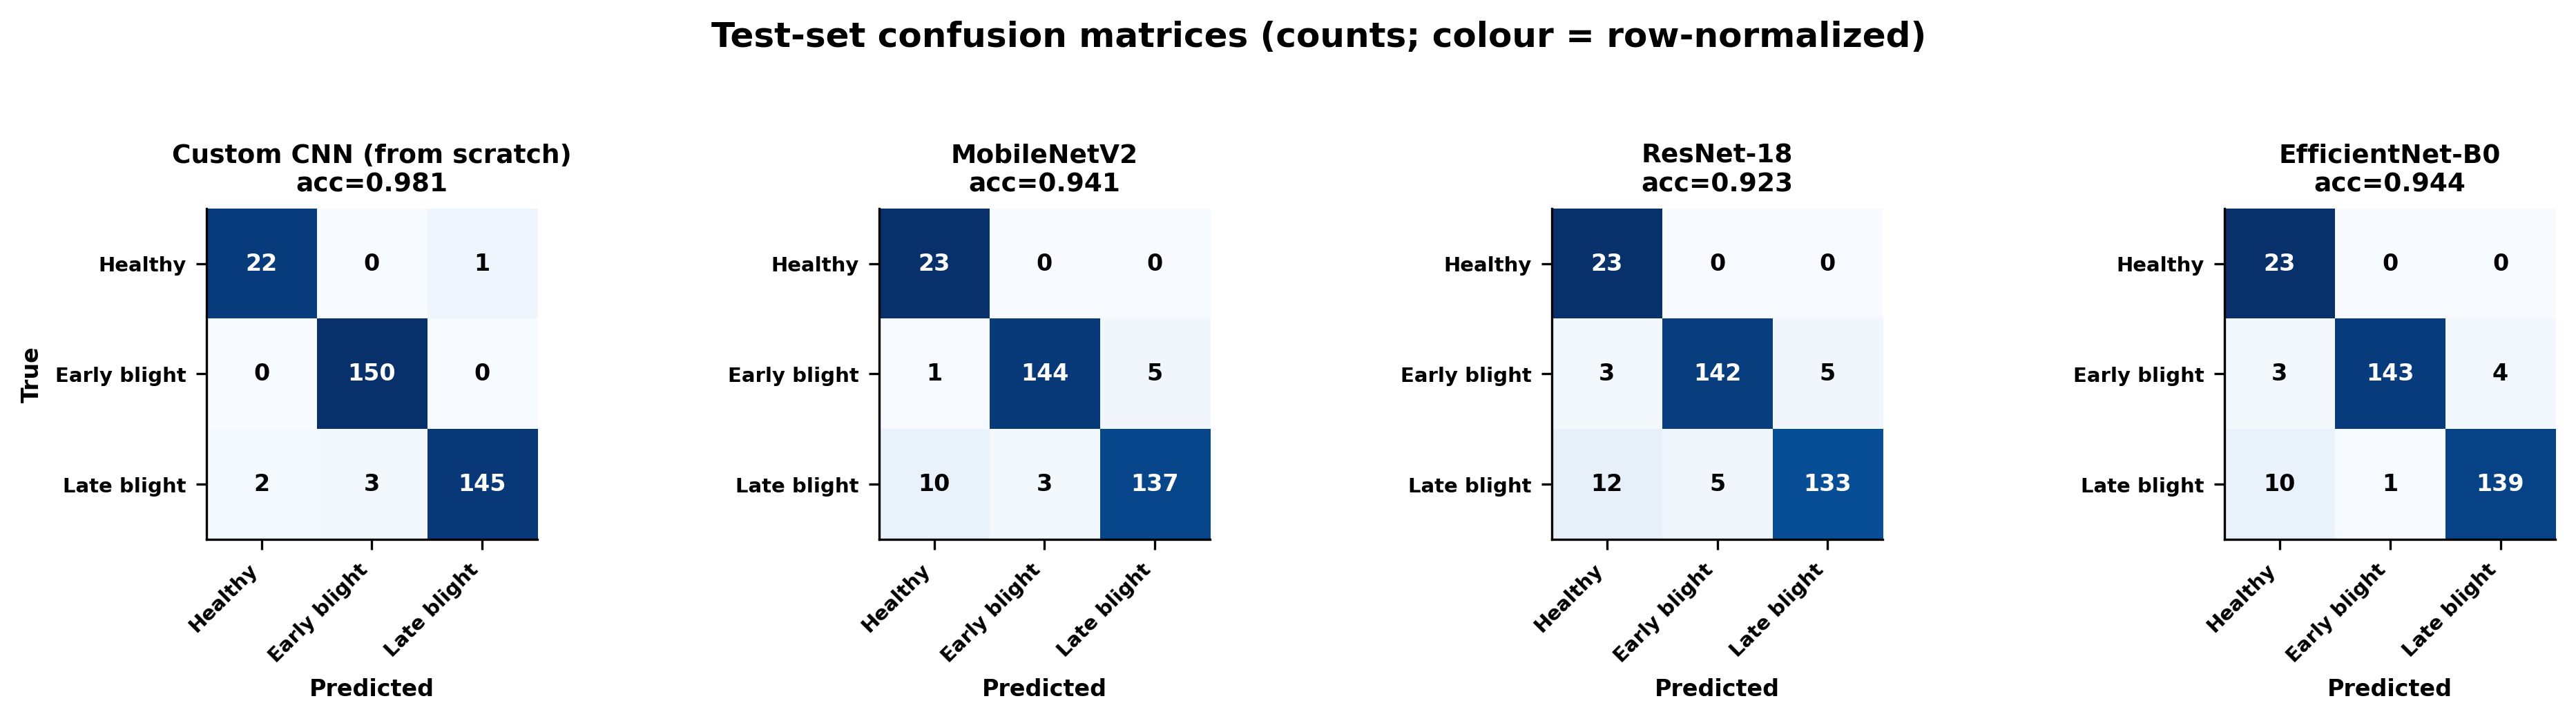
\includegraphics[width=0.98\linewidth]{confusion_matrices.png}}{\fbox{\parbox{0.6\linewidth}{\centering\vspace{1cm}[confusion\_matrices.png]\vspace{1cm}}}}
\caption{Per-model test-set confusion matrices (cell text: counts; colour:
row-normalised rate).}
\label{fig:confusion}
\end{figure}

\subsection{Calibration}
Beyond accuracy, a deployable diagnostic should report trustworthy confidences.
Fig.~\ref{fig:reliability} shows reliability diagrams and ECE values. The custom CNN
attains an ECE of $\eceCustom$, indicating that its softmax confidences track its
empirical accuracy reasonably well, on par with the pretrained baselines. This
matters in practice: a well-calibrated model can defer uncertain cases to a human
expert.

\begin{figure}[t]
\centering
\IfFileExists{figures/reliability_diagrams.png}{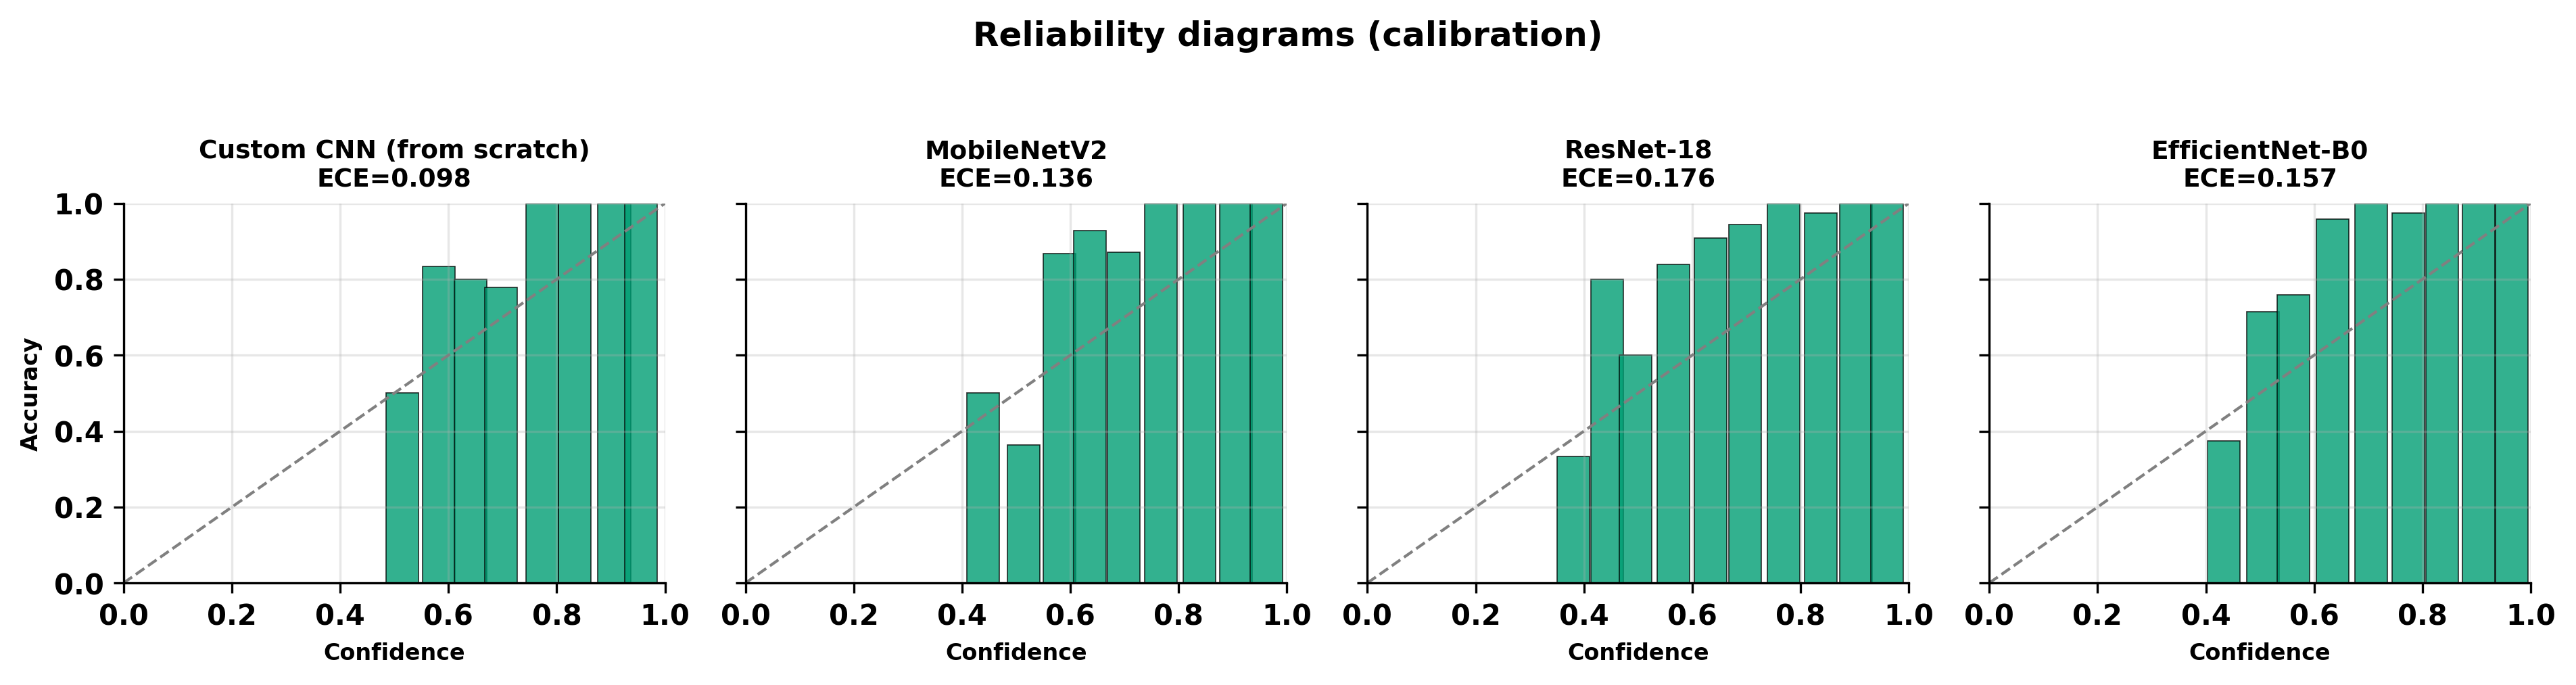
\includegraphics[width=0.98\linewidth]{reliability_diagrams.png}}{\fbox{\parbox{0.6\linewidth}{\centering\vspace{1cm}[reliability\_diagrams.png]\vspace{1cm}}}}
\caption{Reliability diagrams (calibration). The dashed diagonal is perfect
calibration; bars show accuracy within each confidence bin.}
\label{fig:reliability}
\end{figure}

\subsection{Where do the models look?}
Grad-CAM saliency maps (Fig.~\ref{fig:gradcam}) provide the study's most important
qualitative finding. While the models do place attention on visible lesions for the
disease classes, they also assign substantial saliency to leaf margins and to the
uniform background. This is direct visual evidence of the background bias that
Noyan~\cite{noyan2022uncovering} and Barbedo~\cite{barbedo2018impact} warned of: part
of the models' apparent skill derives from dataset artefacts rather than from
pathology. The headline accuracies should therefore be read as an upper bound on
real-world, in-field performance.

\begin{figure}[t]
\centering
\IfFileExists{figures/gradcam_panel.png}{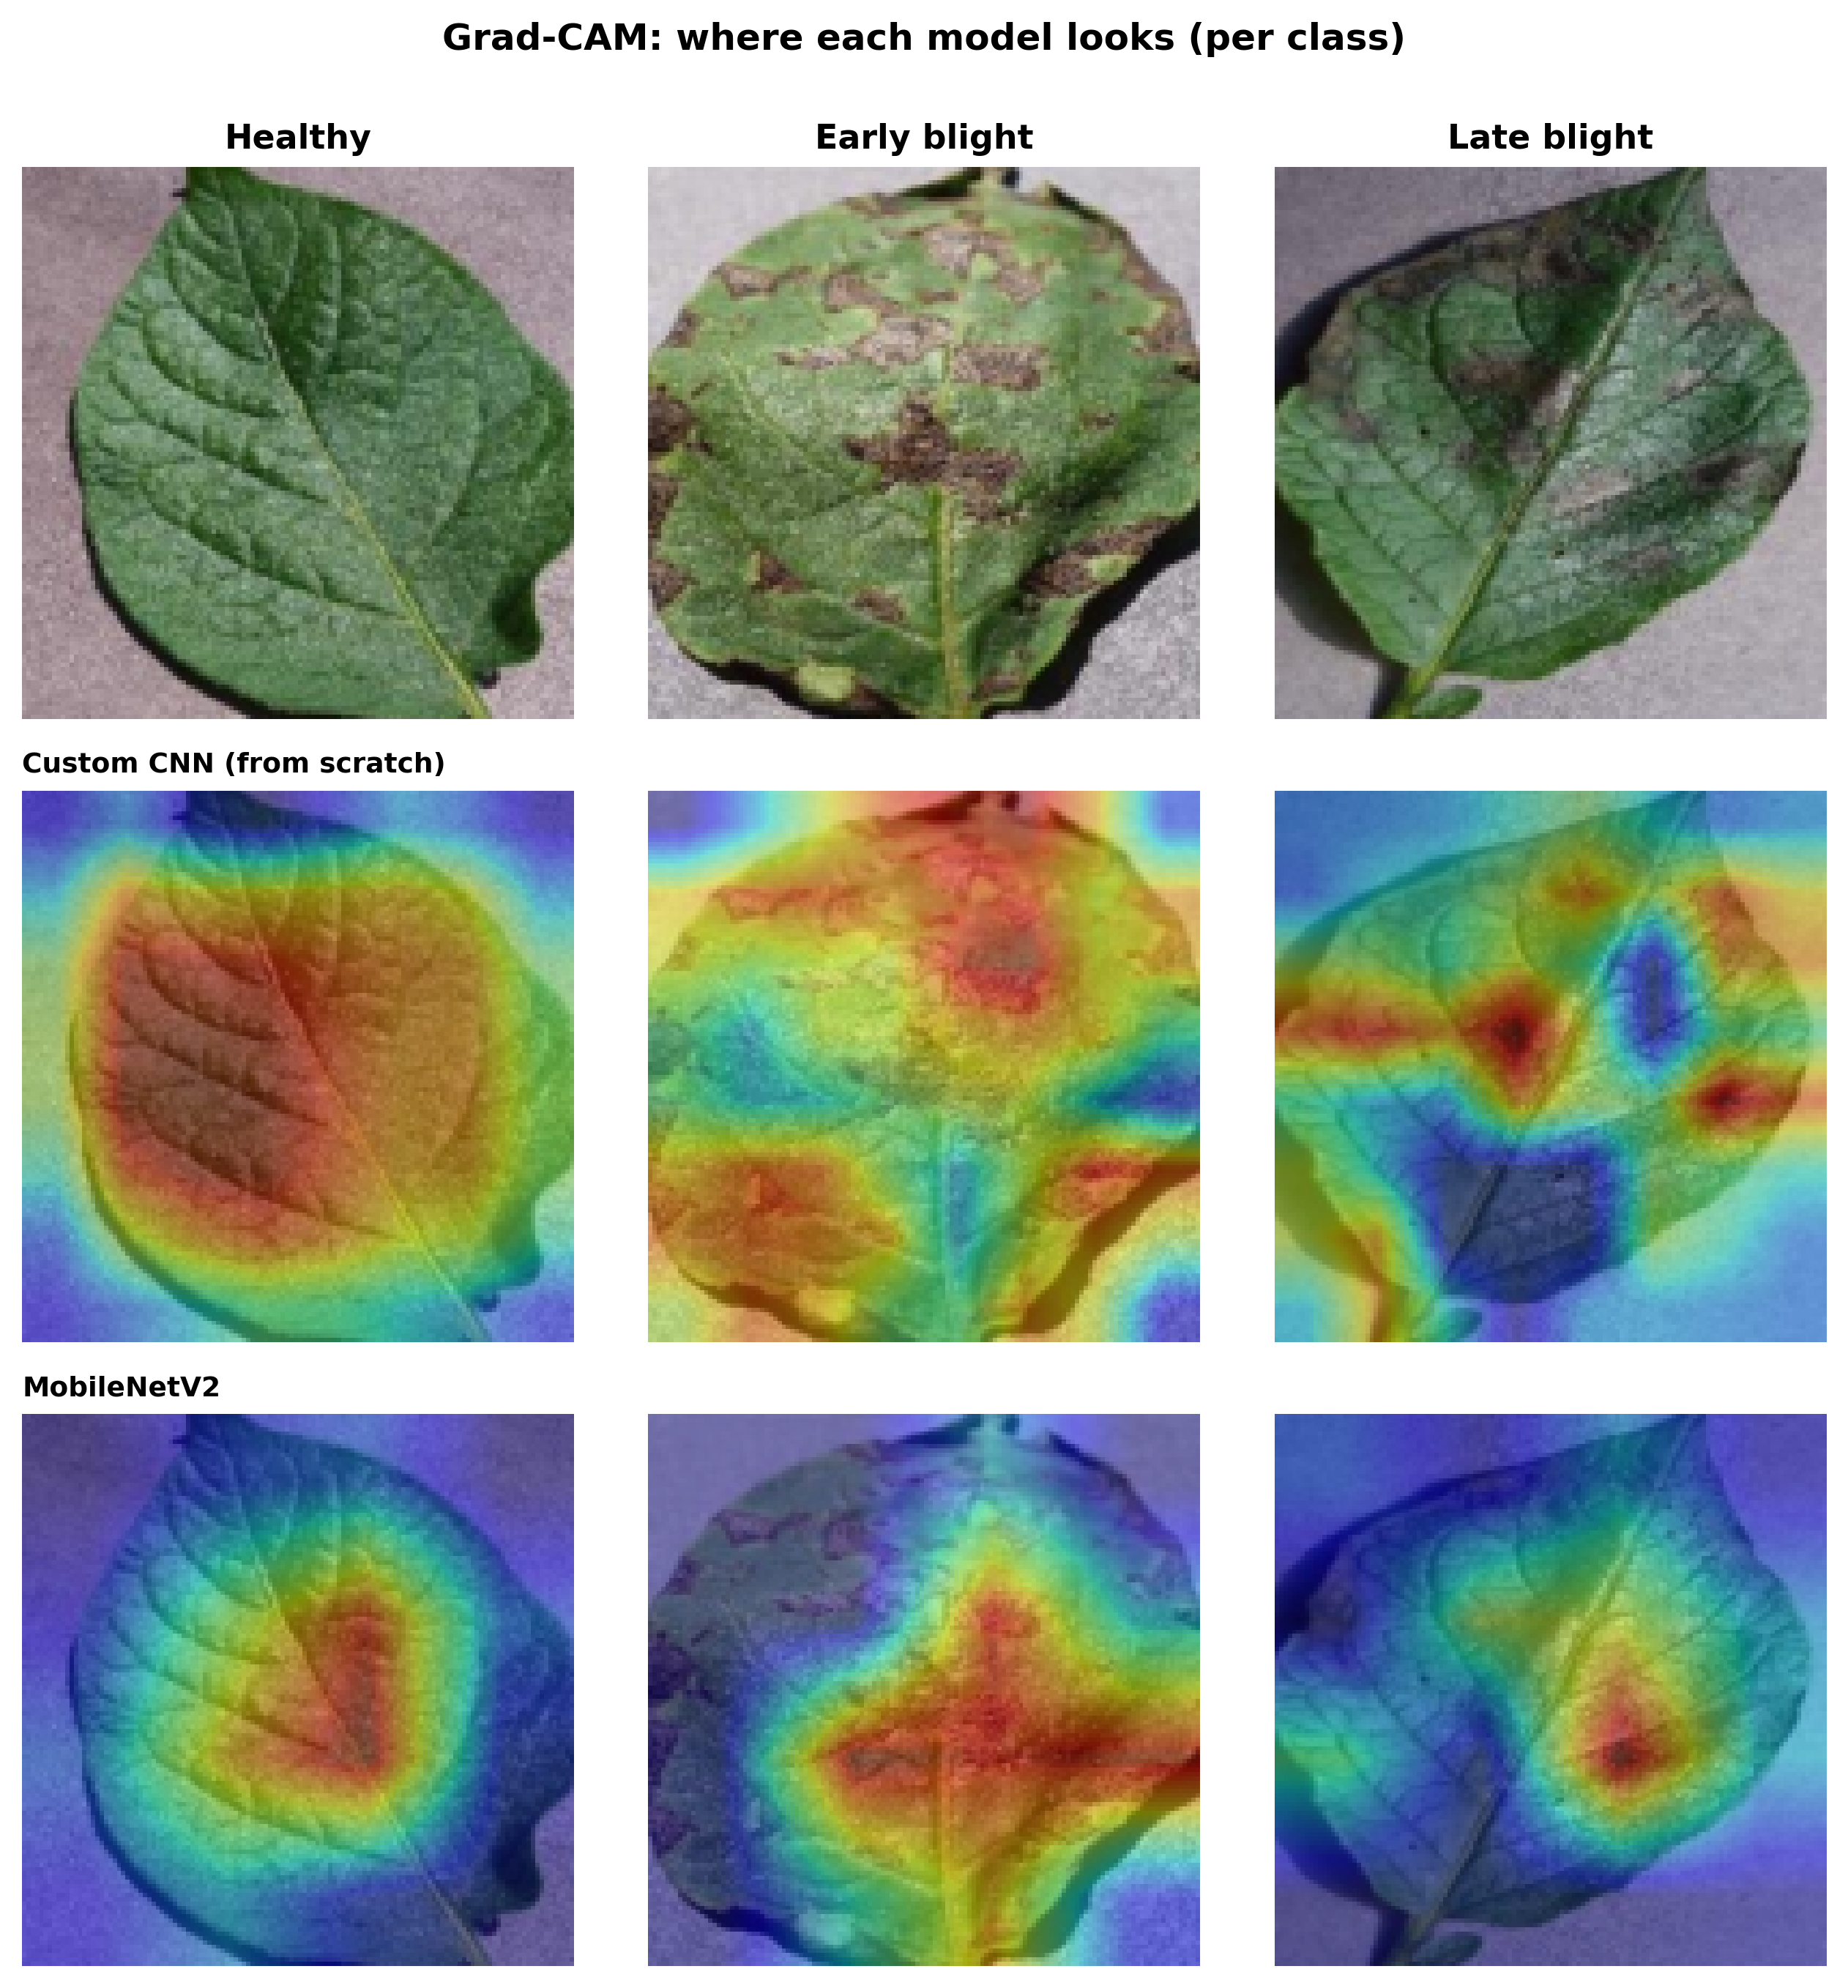
\includegraphics[width=0.95\linewidth]{gradcam_panel.png}}{\fbox{\parbox{0.6\linewidth}{\centering\vspace{1cm}[gradcam\_panel.png]\vspace{1cm}}}}
\caption{Grad-CAM overlays for one example per class. Warm regions are the most
influential for the predicted class. Attention spills onto background, evidencing the
PlantVillage background bias.}
\label{fig:gradcam}
\end{figure}

\section{Discussion}
Our results support a nuanced conclusion. On the one hand, a small CNN trained from
scratch on a laptop is \emph{not} meaningfully outperformed by ImageNet-pretrained
backbones for this three-class problem; transfer learning buys faster convergence
more than higher final accuracy. For practitioners targeting a narrow, well-defined
diagnostic task on accessible hardware, a compact bespoke model is a defensible and
far cheaper choice. On the other hand, the Grad-CAM analysis is a cautionary result
that no amount of additional accuracy on PlantVillage can resolve: because the
dataset's backgrounds are informative, high within-dataset scores do not guarantee
field robustness.

\textbf{Limitations.} The study is deliberately scoped. PlantVillage images are
laboratory captures with clean backgrounds; field images contain clutter, variable
lighting and co-occurring conditions, and we expect all models to degrade on them.
The three-class potato task is comparatively easy, which compresses the differences
between architectures. We freeze the transfer backbones rather than fully fine-tuning
them, trading a little accuracy for speed and a fair, low-compute comparison. We do
not deploy on a mobile device, though the parameter counts suggest feasibility.

\textbf{Future work.} The natural next steps are evaluation on field-collected
potato images, explicit background-removal or segmentation to force the model onto
the leaf, and on-device benchmarking of latency and energy. The reproducible pipeline
released here is designed to make those extensions straightforward.

\section{Conclusion}
We presented a reproducible, statistically careful comparison of a from-scratch CNN
against transfer-learning baselines for potato leaf disease classification on
commodity hardware. The compact custom model is competitive with much larger
pretrained networks, and Grad-CAM reveals a shared reliance on dataset background
that qualifies all reported accuracies. The work argues for honest, interpretable and
hardware-accessible plant-disease modelling over leaderboard chasing.

\section*{Author contributions}
N.P. conceived and designed the study, implemented the data pipeline, models,
training and evaluation code, ran the experiments and statistical analyses, produced
the figures, and wrote and revised the manuscript. As a single-author work, all
contributions are attributable to N.P.

\section*{Data availability}
The PlantVillage dataset is publicly available~\cite{hughes2015plantvillage}. The
download script and the exact potato subset used are described in the code
repository; no image data are redistributed here.

\section*{Code availability}
All code, configurations, pinned dependencies and scripts to reproduce every number
and figure in this manuscript are available at
\url{https://github.com/nielspacheco1997/papa-vision}.

\section*{Competing interests}
The author declares no competing interests.

\bibliographystyle{unsrt}
\bibliography{references}

\end{document}
